
%*******************************************************************************
%*********************************** Second Chapter ***************************
%*******************************************************************************
%!TEX root = 0.main.tex

\section{Non uniform sampling schemes and the FEM Laplacian}

In Chapter 3, we used the fact that when the sampling scheme of the sphere is regular enough, the graph $G$ is such that the corresponding graph Laplacian $\mathbf {L=V\Lambda V}^\intercal$ has eigenvectors that are close enough to the ones of $\Delta_{\mathbb S^2}$ to design a graph with a low mean equivariance error. We showed a way to construct a graph $G'$ such that its graph Laplacian well approximates $\Delta_{\mathbb S^2}$ in the case of an equiarea sampling scheme of the sphere and we tested it on the HEALPix sampling scheme. In this Chapter we focus on sampling schemes that are less uniform than HEALPix. The sampling scheme $V=\{v_i\in \mathbb S^2\}$ that we will use for our study, very used in applications, is the so called \textit{equiangular sampling scheme} \cite{Driscoll:1994:CFT:184069.184073}. 
This chapter is organized as follows: In section \ref{sec:Chapter3: Heat Kernel Graph Laplacian on the Equiangular Sampling} we first introduce the equiangular sampling, and then we present the results that we obtained with two different Graph Laplacians: the HKGL, and a graph proposed by Khasanova et al. \cite{Frossard2017GraphBasedCO}, specifically designed for this sampling scheme. In section \ref{sec:Chapter3: Using the Finite Element Method to approximate the Laplace-Beltrami operator on a manifold} we deepen how to use the Finite Element Method (FEM) to construct a discrete approximation of $\Delta _{\mathbb S^2}$ and how to derive a graph-like Laplacian from it, that shows a low equivariance error.
\subsection{Graph Laplacian on the Equiangular Sampling}
\label{sec:Chapter3: Heat Kernel Graph Laplacian on the Equiangular Sampling}

\subsubsection{The Equiangular Sampling}

Given the usual parametrization $x = x(\theta, \phi)$ of the sphere
\begin{align*}
	\mathbb{S}^{2}&=\left\{x=\left(x_{1}, x_{2}, x_{3}\right) \in \mathbb{R}^{3} :\|x\|_{\mathbb{R}^{3}}=\left(x_{1}^{2}+x_{2}^{2}+x_{3}^{2}\right)^{1 / 2}=1\right\}\\
	x_{1}&=\cos (\phi) \sin (\theta), \quad x_{2}=\sin (\phi) \sin (\theta), \quad x_{3}=\cos (\theta)
\end{align*}

Let $m\in\mathbb N$, the \textit{equiangular sampling} of bandwidth $b=2^m$ is given by 
$
x_{j k}^{(b)}=x\left(\theta_{j}^{(b)}, \phi_{k}^{(b)}\right)
$
where
\begin{align*}
	\theta_{j}^{(b)} &:=\pi \frac{j}{2 b}, \quad \phi_{k}^{(b)} :=2 \pi \frac{k}{2 b}\\
	j&=0, ..., 2b-1 \text{ and }k=0, ..., 2b-1 
\end{align*}

\begin{figure}[h]
	\centering
	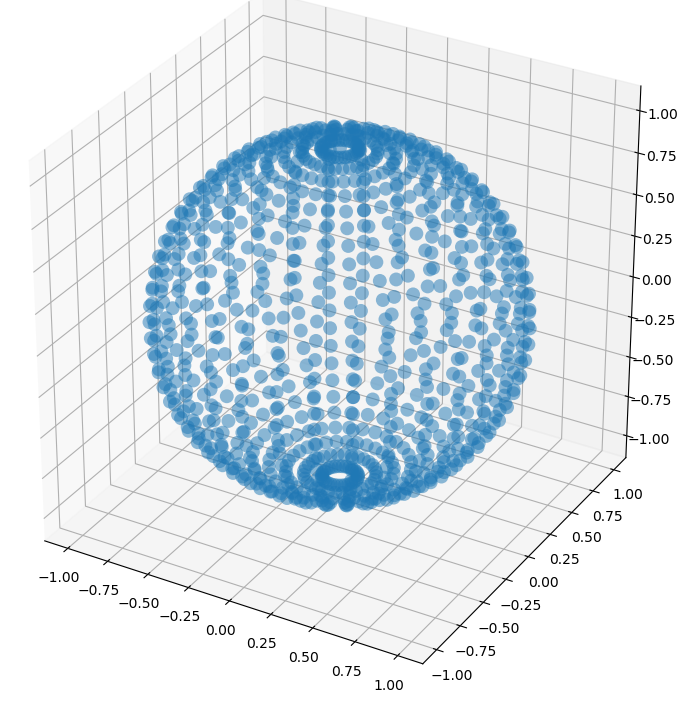
\includegraphics[width=0.5\textwidth]{figs/Chapter3/equiangular.png}
	\caption{\label{fig:equiangular sampling}Equiangular sampling with bandwidth $b=8$}
\end{figure}
One has thus $n=4b^2$ points on the sphere, where all the points $x_{0 k}^{(b)}$ correspond to the north pole for every $k=0, ..., 2b-1$. Notice also that the south pole is never sampled. In figure \ref{fig:equiangular sampling} it can also be appreciated how the area close to the poles is much more sampled that the equator. One reason for which this sampling scheme is very used in application is the existence of the following result from \cite{Driscoll:1994:CFT:184069.184073}, that states that any band limited function can be exactly recovered from its sampled values $f\left(x_{j k}^{(b)}\right)$:
\vspace{0.5cm}
\begin{theorem}\label{theo:equiangular sampling theorem}
	Let \(l_{0} \in \mathbb{N}\) and \(m_{0} \in \mathbb{Z},\left|m_{0}\right| \leq l_{0} .\) If \(f=\sum_{l=0}^{b-1} \sum_{m=-l}^{l} \widehat{f}(l, m) Y_{l}^{m}\)
	then
	
	$$
	\begin{aligned} \widehat{f}\left(l_{0}, m_{0}\right)=& \frac{1}{4 b^{2}} \sum_{j=0}^{2 b-1} \sum_{k=0}^{2 b-1} f\left(x_{j k}^{(b)}\right) \overline{Y_{l_{0}}^{m_{0}}\left(x_{j k}^{(b)}\right)} \sin \left(\theta_{j}^{(b)}\right) \times \\ & \times \frac{4}{\pi} \sum_{l=0}^{b-1} \frac{1}{2 l+1} \sin \left((2 l+1) \theta_{j}^{(b)}\right) \end{aligned}
	$$
\end{theorem}
\vspace{0.5cm}
Theorem \ref{theo:equiangular sampling theorem} is the equivalent on the sphere of the well known Shannon's sampling theorem, that states the minimum sampling frequency at which a band limited signal $f:\mathbb R \to \mathbb R$ can be perfectly reconstructed, and is a precious tool when doing signal processing on the sphere.

\subsubsection{Heat Kernel Graph Laplacian on the equiangular sampling scheme}
Thanks to theorem \ref{theo:equiangular sampling theorem} not only we have a characterization of the space \\$F=\{f=\sum_{l=0}^{b-1} \sum_{m=-l}^{l} \widehat{f}(l, m) Y_{l}^{m}\}\subset L^2(\mathbb  S^2)$ of band limited functions on which the sampling operator $T: F\to \mathbb R^n$ is invertible, but we also an analytic expression for $T^{-1}$. Thanks to this we can calculate up to machine precision the equivariance error for any function $f\in F$ and any rotation $g\in SO(3)$. In figure \ref{fig:Equivariance error of the full HKGL} we calculated the mean equivariance error of the full HKGL averaging on mono-frequency signals for different bandwidths. We can observe a much cleaner behavior of the mean equivariance error than the one we observed for he HEALPix sampling, most probably due to the fact that this time we can exactly calculate $T^{-1}$. The error increases linearly with the frequency of the signal for all bandwidths, and it seems to converge to zero as $b$ increases. However, the spectrum of the graph Laplacian does not show the eigenvalues grouped in the expected pattern.
\begin{table}[h!]
	\centering
	\begin{tabular}{ c|c } 
$b$ & $t$ \\ 
	\hline
4 & 0.5 \\ 
8 & 0.3 \\ 
16 & 0.1 \\ 
	\end{tabular}
	\caption{\label{table:equiangular kernel width}Kernel width $t$ used to construct the HKGL for each bandwidth $b$}
\end{table}

\begin{figure}[h!]
	\centering
	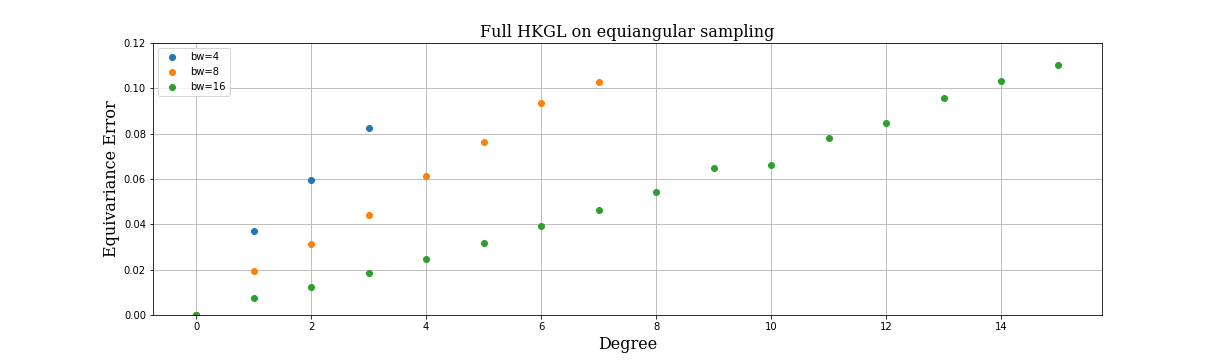
\includegraphics[width=\textwidth]{../codes/06.Equivariance_error/FullHKGLonequiangularsampling.png}
	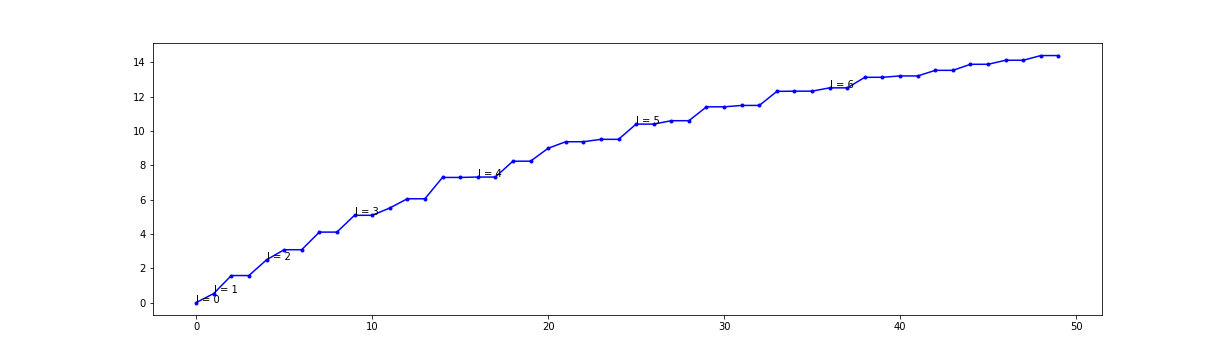
\includegraphics[width=\textwidth]{../codes/02.HeatKernelGraphLaplacian/equiangular/equi_full_eigenvalues_16.png}
	\caption{\label{fig:Equivariance error of the full HKGL}Equivariance error of the full HKGL on the equiangular sampling by spherical harmonic degree $\ell$, and its spectrum for the bandwidth $b=8$ .}
\end{figure}

\subsubsection{A graph alternative to the HKGL for the equiangular sampling}\label{sec:Chapter3:Frossard}

Khasanova et al. \cite{Frossard2017GraphBasedCO} designed a discrete Laplacian that is explicitly intended to work on the sphere with the equiangular sampling. They studied a way to build a graph to analyze images produced by omnidirectional cameras. In their work they assume that the image is sampled on the sphere on the equiangular sampling. They consider the set $\mathcal G$ of all the possible graphs where each node is connected only to four of its nearest neighbours (North, Sud, West, East) and propose a weighting scheme $w_{ij}$ that minimizes the difference in the response to the polynomial spectral filter $\mathcal F = \mathbf L$ evaluated on images of the same object seen at different latitudes. In other words, they solve the minimization problem

\begin{equation}\label{eq:minimization frossard}
	\min_{W\in\mathcal G} \left|\mathcal{F}\left(\mathbf{y}\left(v_{ e}\right)\right)-\mathcal{F}\left(\mathbf{y}\left(v_{ i}\right)\right)\right|
\end{equation}
\begin{figure}
	\begin{center}
		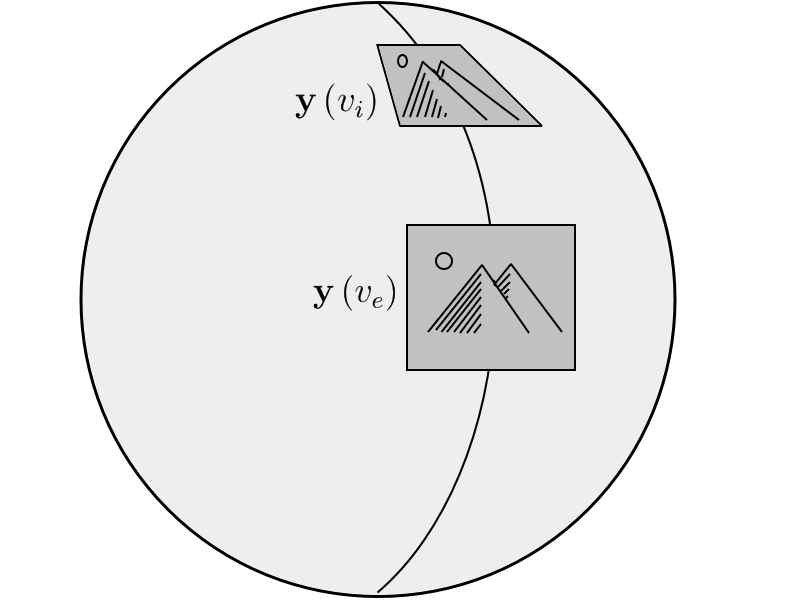
\includegraphics[width=0.5\textwidth]{figs/Chapter3/frossard2.png}
	\end{center}
	\caption{\label{fig:frossard2}Khasanova et al. setting.}
\end{figure}
for the adjacency matrix $W$, where $\mathbf y(v_i)$ is the image of the object on the sphere centered on the vertex $v_i$, and $\mathcal F (\mathbf y(v_e))$ is the response of the filter at the vertex $v_e$ that lies at the same longitude of the vertex $v_i$ but on the equator (figure \ref{fig:frossard2}). In their work they prove that the optimal weights solving the minimization problem (\ref{eq:minimization frossard}) are given by weights $w_{ij}$ inversely proportional to the Euclidean distance between vertices:
\begin{equation}\label{eq:frossard weights}
	w_{ij} = \frac{1}{\norm{x_i-x_j}}
\end{equation}
This construction is interesting since it is adapted to the equiangular sampling, and leads to a very sparse graph with only 4 neighbors per vertex. Furthermore, to obtain the weights (\ref{eq:frossard weights}) every calculation was done in the \textit{spatial domain}, without any consideration about the spectral interpretation of the filter. In order to compare it to the HKGL we show the equivariance error by spherical harmonic degree in figure \ref{fig:Equivariance error of the Frossard-Khasanove graph}. It can be appreciated how this construction performs a little worse that the full HKGL for low bandwidth samplings, but converges faster than the \textit{full} HKGL, and its spectrum looks much more similar to the one of $\Delta_{\mathbb S^2}$.

\begin{figure}[h!]
	\centering
	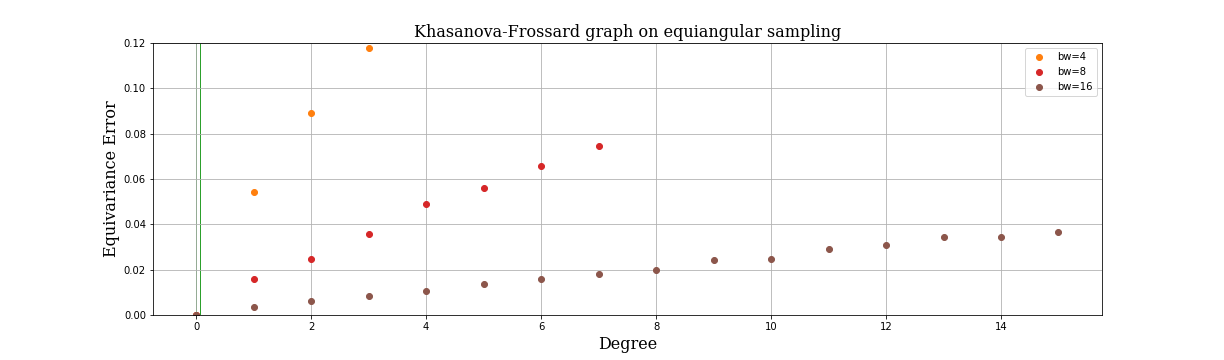
\includegraphics[width=\textwidth]{../codes/06.Equivariance_error/KhasanovaFrossardgraphonequiangularsampling.png}
	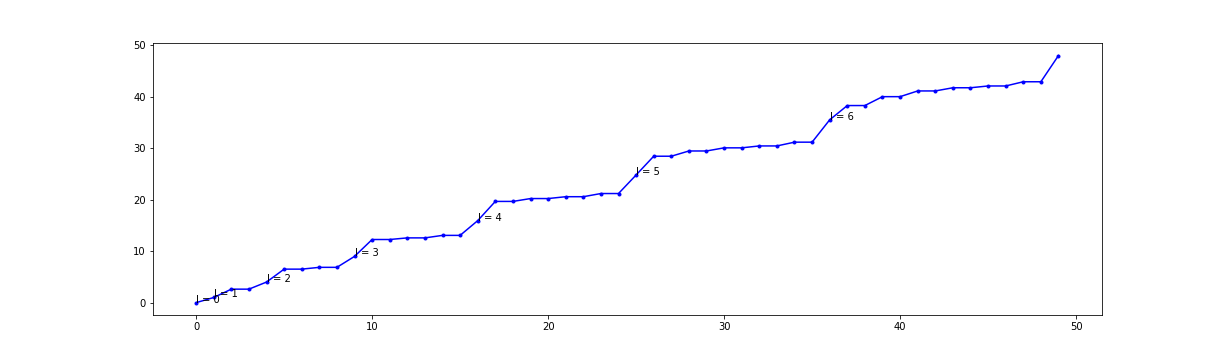
\includegraphics[width=\textwidth]{../codes/02.HeatKernelGraphLaplacian/equiangular/equi_full_Khasanova_Frossard_eigenvalues_16.png}
	\caption{\label{fig:Equivariance error of the Frossard-Khasanove graph}Equivariance error of the Khasanova-Frossard graph on the equiangular sampling with bandwidth $b=8$ by spherical harmonic degree $\ell$, and its spectrum.}
\end{figure}

The Khasanova-Frossard graph showed us that it is possible to do better than the HKGL on the equiangular sampling. We asked ourself if there's a general way of building a more equivariant graph than the HKGL that is straightforward to implement on any sampling scheme of the sphere. To answer this question in the next section we study a more complex way to approximate the Laplace-Beltrami operator $\Delta_{\mathbb S^2}$: the linear FEM Laplacian. We will see that the comparison between the FEM Laplacian and the graph Laplacian will give us precious insights to better understand the limitations of graph Laplacians when it comes to deal with non uniform samplings of the sphere.
\subsection{The Finite Element Method approximation of the Laplace-Beltrami operator on the sphere}\label{sec:Chapter3: Using the Finite Element Method to approximate the Laplace-Beltrami operator on a manifold}

The Finite Element Method (FEM) is a numerical algorithm that allows to calculate a discrete approximation of the solution of the Laplace-Beltrami eigenvalue problem through a functional discretization of the differential operator $\Delta_{\mathbb S^2}$.  We put the necessary definitions and mathematical concepts necessary to properly introduce the weak formulation of a differential problem, the Galerkin method and finally the Finite Element Method in Appendix. For a detailed introduction to the FEM, we refer the reader to \cite{Quarteroni:1639539}\\
Let's transform the strong form of the eigenvalue problem on the Sphere on its \textit{weak} formulation. Let's multiply equation (\ref{eq:continous eigenvalue problem}) by a sufficiently regular function $v$ and integrate on $\mathbb S^2$. Since the sphere is a closed manifold and has no border, integrating by parts yields
\begin{equation}\label{eq:weak eigenvalue problem}
\begin{split}
&\text{Find } f\in H^1(\mathbb S^2), \lambda\in\mathbb R\text{ such that }\\ 
&\int_{\mathbb S^2} \nabla f(\mathbf x)\cdot\nabla v(\mathbf x) d\mathbf x = \lambda \int_{\mathbb S^2} f(\mathbf x)\cdot v(\mathbf x)d\mathbf x\quad \forall v\in H^1(\mathbb S^2)
\end{split}
\end{equation}
where $v$ has been chosen to belong to $H^1\subset L^2(\mathbb S^2)$, the Sobolev space of all the functions with derivative $\nabla f\in L^2(\mathbb S^2)$. The Finite Element Method first approximates the domain $\Omega$ with a triangulation $\mathcal T_h=\{ \tau_i \}$, and then \textit{projects} the weak problem (\ref{eq:weak eigenvalue problem}) into a finite dimensional subspace $V_h\subset H^1(\mathcal T_h)$ made by all the piecewise linear polynomials on the triangulation $\mathcal T_h$. Being the sphere convex, the triangulation $\mathcal T_h$ has been obtained by calculating the triangulation of the convex hull of the vertices of the chosen sampling scheme through the Qhull algorithm \cite{Barber96thequickhull}. Now, define $X_h^1$ to be the space of all the continuous, piecewise linear functions on $\Omega$
$$X_h^{1}=\{v_h: v_h\in C(\Omega): \left.v_h\right|_{\tau}\in\mathbb P^1\  \forall \tau\in \mathcal T_h\}$$ 
and set $V_h=X_h^1$. Since for the functions in $X_h^1$ the number of degrees of freedom is the same of the number of vertices of the mesh $n$, we need  $n$ basis functions $\phi_i, i=0,...,n-1$ to fully describe $X_h^{1}$. $\phi_i$ is defined as the continuous piecewise linear function such that 
$$
\phi_i(x_j) = \delta_{ij}\quad i=0,...,n-1
$$
where $x_i$ are the points of the sampling scheme that have been used as vertices of the triangles $\tau$ of the triangulation $\mathcal T_h$. The support of $\phi_i$ i.e., the subset of $\mathcal T_h$ where $\phi_i$ is not zero, is made by all the triangles sharing the $i$th vertex. An example is shown in figure \ref{fig:basis function}.

\vspace{0.5cm}
\begin{remark}
	For a function $v_h \in X^1_h,\ v_h = v_0 \phi_0 +...  v_n \phi_n$ the coefficient $v_i$ is equal to the function $v_h$ evaluated in the $i$th vertex 
	\begin{equation}\label{eq:dof and values}
	v_i = v_h( x_i)
	\end{equation}
\end{remark}\vspace{0.5cm}
\begin{figure}[h]
	\begin{center}
		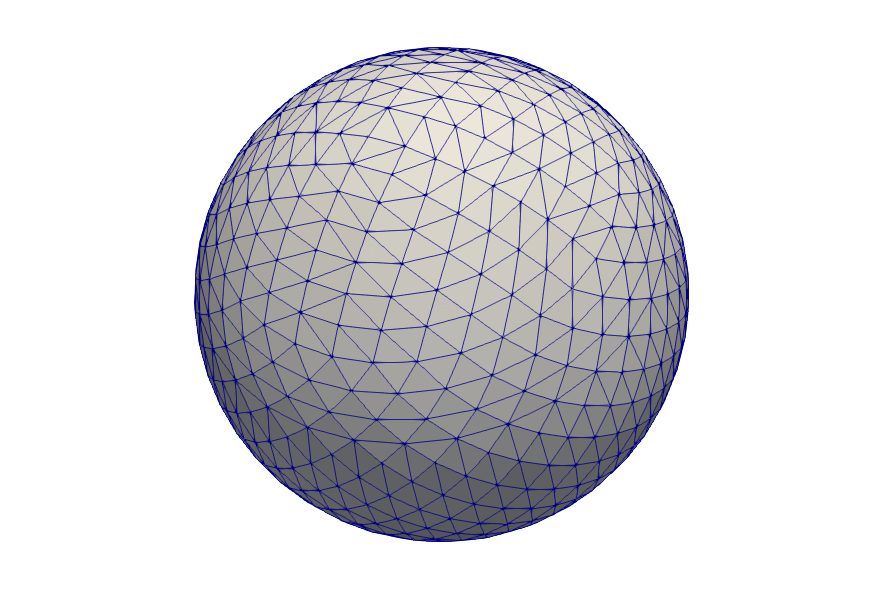
\includegraphics[width=0.6\textwidth]{figs/Chapter3/sphere_mesh.png}
	\end{center}
	\caption{\label{fig:sphere mesh}A triangulation $\mathcal T_h$ of the sphere made with the vertices of the HEALPix sampling scheme with $N_{side}=8$.}
\end{figure}
\begin{figure}
	\begin{center}
		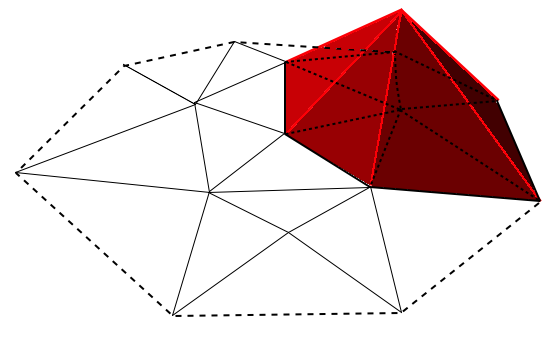
\includegraphics[width=0.4\textwidth]{figs/Chapter3/basisfunction.png}
	\end{center}
	\caption{\label{fig:basis function}Basis function of the space $X^{1}_h$}
\end{figure}

By writing $n$ times the equation (\ref{eq:weak eigenvalue problem}), setting each time the test function $v_h$ equal to the $i$th basis function $\phi_i$ of the space $X_h^1$, we obtain the generalized algebraic eigenvalue problem
\begin{equation}\label{eq:algebraic generalized eigenvalue problem}
\begin{aligned}
&\text{Find }(f,\lambda)\text{ such that }\mathbf A\mathbf f = \lambda\mathbf  B \mathbf f\\
&\begin{cases}
(\mathbf A)_{ij} &= \int_{\mathbb S^2}\nabla \phi_i(\mathbf{x})\cdot \nabla \phi_j(\mathbf{x})d\mathbf{x}\\
(\mathbf B)_{ij} &= \int_{\mathbb S^2} \phi_i(\mathbf{x}) \phi_j(\mathbf{x})d\mathbf{x}\\
(\mathbf f)_i &= f_i:\quad f(\mathbf x) = f_0\phi_0(\mathbf x)+ ... + f_{n-1}\phi_{n-1}(\mathbf x) 
\end{cases}
\end{aligned}
\end{equation}
$\mathbf A$ is called the \textit{stiffness} matrix, and $\mathbf B$ is called the \textit{mass} matrix. Observe that being the Laplace-Beltrami operator self-adjoint, we have that $\mathbf A=\mathbf A^\intercal,$ $\mathbf B=\mathbf B^\intercal$. Being $\mathbf B$ non singular, the system (\ref{eq:algebraic generalized eigenvalue problem}) is equivalent to the eigenvalue problem
\begin{equation}\label{eq:algebraic  eigenvalue problem}
\mathbf B^{-1}\mathbf A\mathbf f = \lambda \mathbf f
\end{equation}

It can be shown \cite{Strang} that even though the matrix $\mathbf B^{-1}\mathbf A$ is not symmetric, its eigenvalues are still real and its eigenvectors are such that $\mathbf V\mathbf B\mathbf V^\intercal=\mathbf I$, where $\mathbf I$ is the identity matrix. The solution $\mathbf f$ that is the vector of the coefficients of the function $f_h$ in the basis $\phi_i$ corresponds exactly to the values of the function $f_h$ in the vertices. 

\subsection{How to filter a signal with the linear FEM}
Calculating the discrete Fourier transform with the linear FEM means projecting the Fourier transform into the subspace $V_h$:

\begin{equation}\label{eq:FEM fourier}
	\hat f_{FEM} (\ell, m) = \int_{\eta \in \mathcal T_h} f_h(\eta) v_{i(\ell, m)}(\eta) d\eta = \mathbf v_{i(\ell, m)}^\intercal \mathbf B \mathbf f
\end{equation}

where $ v_{i(\ell, m)}$ is the solution to the eigenvalue problem (\ref{eq:algebraic generalized eigenvalue problem}), $f_h$ is the projection of $f$ on $V_h$, and $\mathbf B$ is the mass matrix. It follows that the filtering of a discretized signal $\mathbf f$ in the spectral domain is done by the following matrix  $\mathbf \Omega_K^{FEM}$:

\begin{equation}\label{eq:FEM filtering}
	 \mathbf \Omega_K^{FEM} := (\mathbf B\mathbf V^\intercal)^{-1}\mathbf K\mathbf V^\intercal\mathbf B
\end{equation}

where $\mathbf V^\intercal\mathbf B$ is the FEM Fourier transform matrix, $\mathbf K$ is the diagonal matrix that represent the chosen kernel for this filter, and $(\mathbf V^\intercal\mathbf B)^{-1}$ is the matrix representing the inverse FEM Fourier transform. We can already notice a fundamental difference between this way of filtering a signal and the way of filtering a signal with a graph. The FEM filtering uses not only the eigenvectors of the FEM Laplacian, but also the mass matrix $\mathbf B$. We computed the usual mean equivariance error per spherical harmonic degree for the diffusion filter $\mathbf K=\exp(-\mathbf \Lambda)$ on the equiangular sampling, and we show it in figure \ref{fig:FEM diffusion}.
\begin{figure}[h]
	\centering
	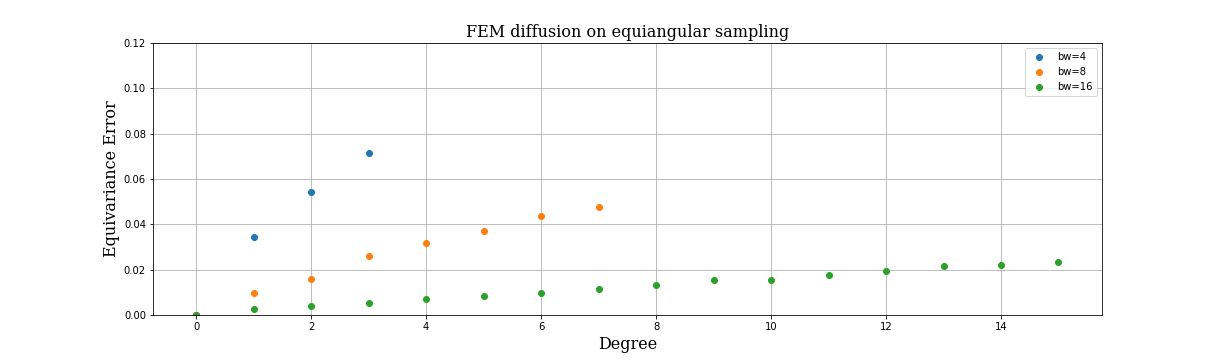
\includegraphics[width=\textwidth]{../codes/06.Equivariance_error/FEMdiffusiononequiangularsampling.png}
	\caption{\label{fig:FEM diffusion}Equivariance error of the linear FEM diffusion on the equiangular sampling by spherical harmonic degree.}
\end{figure}
We can see that the FEM filtering works better than the state-of-the-art graph of Khasanova-Frossard, but the matrix $\mathbf \Omega_K^{FEM}$ is full, and its computation requires the expensive inversion of the Fourier matrix $\mathbf V^\intercal\mathbf B$, making it not efficient if used in a CNN. 
\subsubsection{A confront between FEM filtering and graph filtering}\label{sec:FEM filtering as a graph filtering}
Due to the fact that 
$
\mathbf V^\intercal\mathbf B\mathbf V = \mathbf I
$,
we have that 
$$
\begin{aligned}
	(\mathbf V^\intercal\mathbf B)^{-1} &= \mathbf V,\\
	\mathbf V^\intercal\mathbf B &= \mathbf V^{-1}.
\end{aligned}
$$
So, the FEM filter matrix $\mathbf \Omega_K^{FEM}$ can be rewritten as 
\begin{equation}\label{eq:FEM filter simple}
	 \mathbf \Omega_K^{FEM}  = \mathbf V \mathbf K \mathbf V^{-1}
\end{equation}
Thus a polynomial filter
$$
k(\lambda)=P_\kappa(\lambda) = \sum_{k=0}^{\kappa-1} \theta_k \lambda^k
$$
would be implemented with a matrix
$$
\mathbf\Omega_K^{FEM} = \mathbf V \left(\sum_{k=0}^{\kappa-1} \theta_k \mathbf \Lambda^k \right)\mathbf V^{-1} = \sum_{k=0}^{\kappa-1} \theta_k (\mathbf B^{-1}\mathbf A)^k = P_\kappa(\mathbf B^{-1}\mathbf A).
$$

It is interesting to notice that FEM filtering (\ref{eq:FEM filter simple}) looks very much like graph filtering (\ref{eq:graph convolution}) but, given that $V$ is not orthogonal anymore, it has to replace the $\mathbf V^\intercal$ with $\mathbf V^{-1}$. Equation \ref{eq:FEM filter simple} implies that the FEM filtering could be implemented exactly as the graph filtering already implemented in DeepSphere, using the FEM matrix $\mathbf B^{-1}\mathbf A$ instead of the usual symmetric HKGL $\mathbf L_n^t$. Unfortunately, in order to make the evaluation of the polynomial $P_\kappa(\mathbf B^{-1}\mathbf A)$ efficient, we need the matrix $\mathbf B^{-1}\mathbf A$ to be sparse. The only way to do so is to have a \textit{sparse stiffness matrix} $\mathbf A$ and a \textit{diagonal mass matrix} $\mathbf B$. Unfortunately there is no likely way to have both these conditions satisfied at the same time, since this is one of the most well known trade offs of the FEM \cite{Strang}. To make $\mathbf B$ diagonal we need to choose $\phi_i$ to be an orthogonal basis of the finite dimensional functional space $V_h$. To do so, we will need to choose more complicated basis functions than the usual ones in figure \ref{fig:basis function}, \textit{most likely with a support that extends to the whole sphere}, making the stiffness matrix $\mathbf A$ not sparse anymore. A common workaround \cite{Strang} is the so called \textit{lumping} of the mass matrix, that consists in replacing the matrix $\mathbf B$ with the \textit{lumped} diagonal matrix $\mathbf D$ obtained by placing in each diagonal entry $(\mathbf D)_{ii}$ the sum of the elements of the $i$th row of the mass matrix $\mathbf B$:

\begin{equation}\label{eq:lumping}
\mathbf D = \text{diag}\{d_i\},\quad d_i = \sum_j (\mathbf B)_{ij}
\end{equation}
This approximation is well studied in the literature and it is proved to work well in many practical cases \cite{Quarteroni:1639539}. In this way the FEM matrix $\mathbf B^{-1}\mathbf A$ would be approximated by the matrix
$$
\mathbf D^{-1}\mathbf A.
$$
This matrix has the big advantage of having the same sparsity pattern of the stiffness matrix $\mathbf A$, making it very efficient for polynomial filtering. We can take one step further by using the symmetric matrix
$$
\mathbf D^{-1/2}\mathbf A\mathbf D^{-1/2}.
$$
To confront FEM and HKGL filtering we filter a unit mass signal \\$\mathbf{f}=(0,0,...0,1,0,...,0)^\intercal$ with the \textit{diffusion} filter $\exp{(-\tau \mathbf L)}$. It was chosen a very irregular sampling scheme, shown in figure \ref{fig:FEM lumped symmetric diffusion on irregular sampling}. It can be seen how the full HKGL compresses the signal around the equator where the sampling scheme is more sparse; on the other hand the FEM filtering manages to keep the diffusion homogeneous no matter the asymmetry in the sampling scheme. 
The mean equivariance error using by spherical harmonic degree can be found in figure \ref{fig:Equivariance error of the lumped FEM Laplacian}. It can be seen how $\mathbf D^{-1}\mathbf A$ ha almost the same equivariance error of the full FEM Laplacian $\mathbf B^{-1}\mathbf A$, while using the symmetric matrix $\mathbf D^{-1/2}\mathbf A \mathbf D^{-1/2}$ makes the equivariance error much worse, especially at lower frequencies.
\clearpage
\begin{figure}[h!]
	\centering
	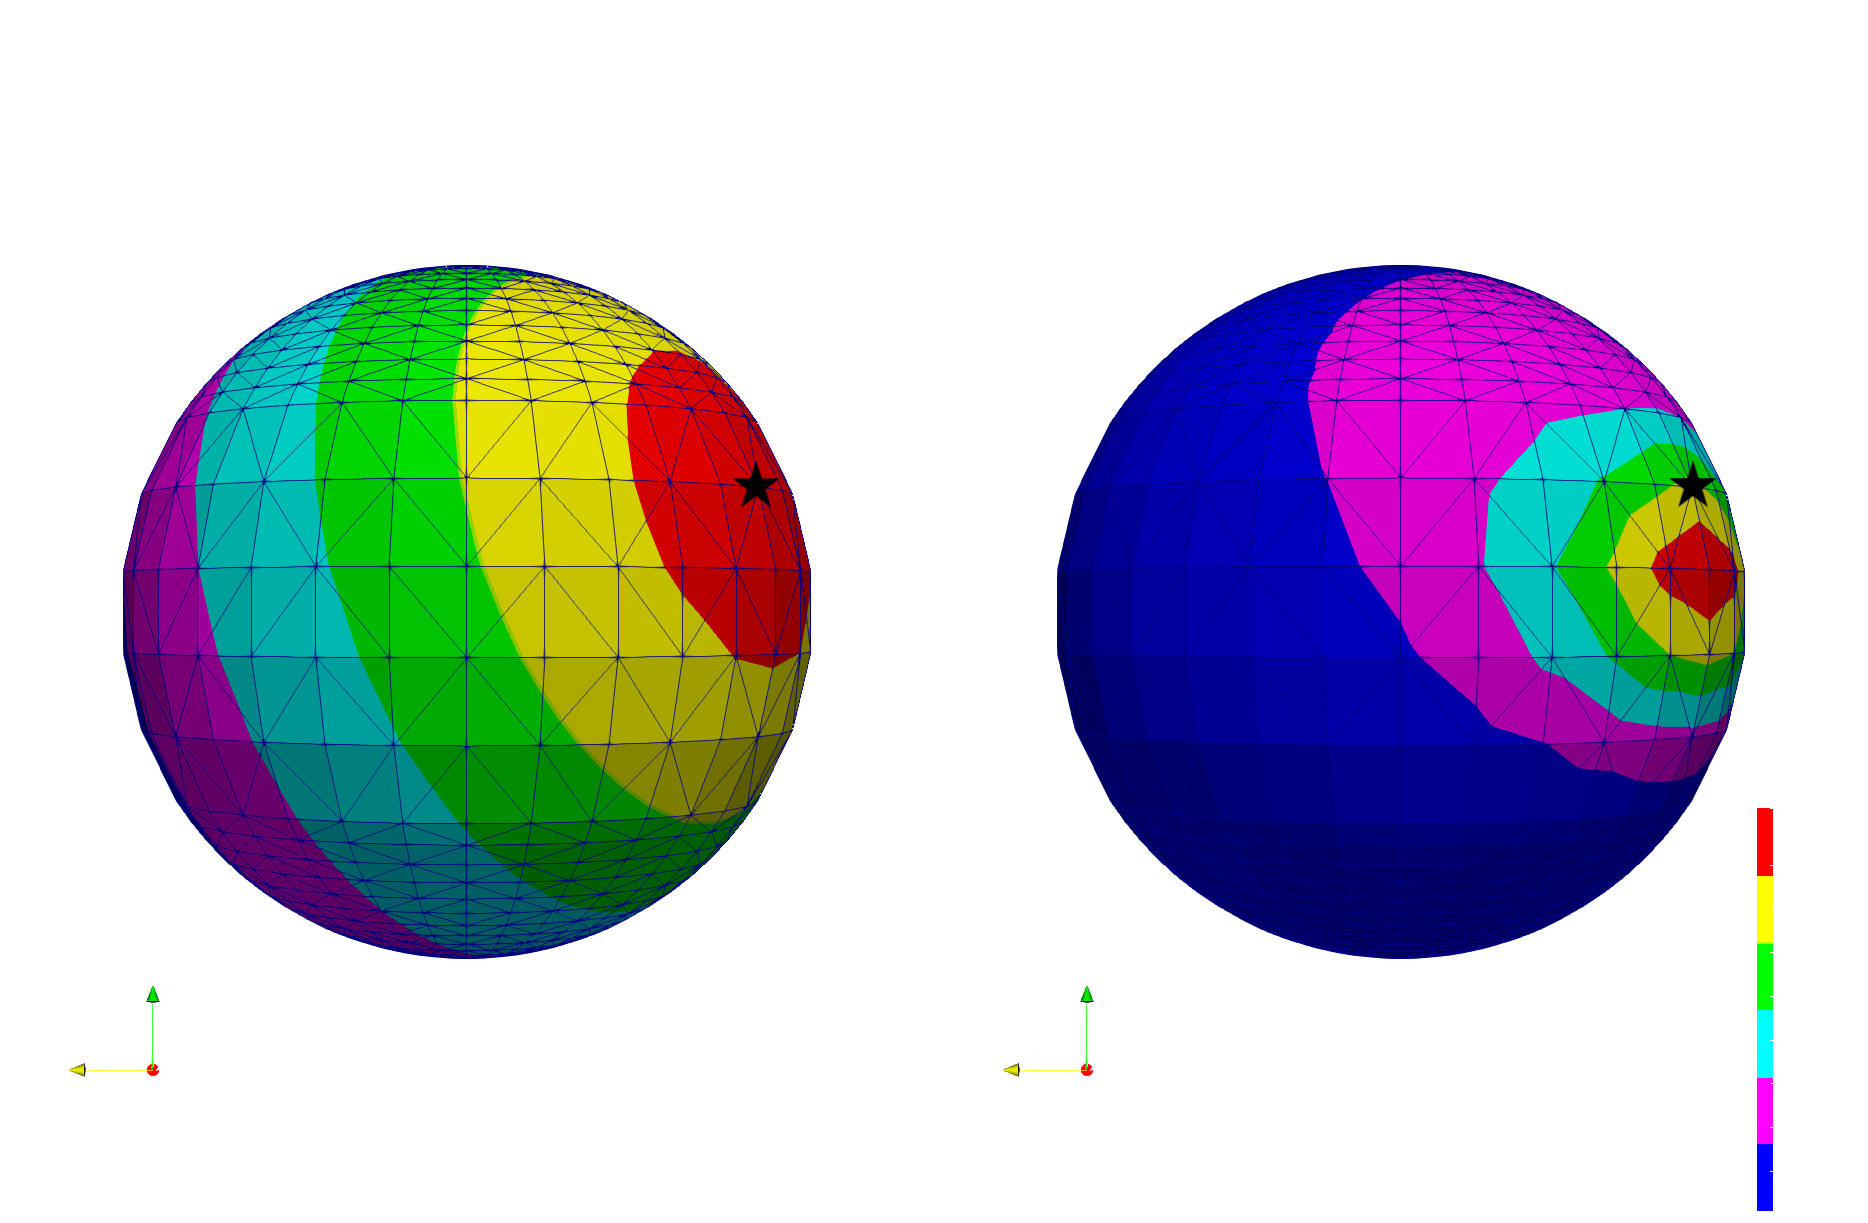
\includegraphics[width=\textwidth]{figs/Chapter3/diffusion.png}
	\caption{\label{fig:FEM lumped symmetric diffusion on irregular sampling}Symmetric lumped linear FEM diffusion and HKGL diffusion on an irregular sampling scheme of the sphere. The position of the filtered source signal is indicated with a black star.}
\end{figure}
\begin{figure}[h!]
	\centering
	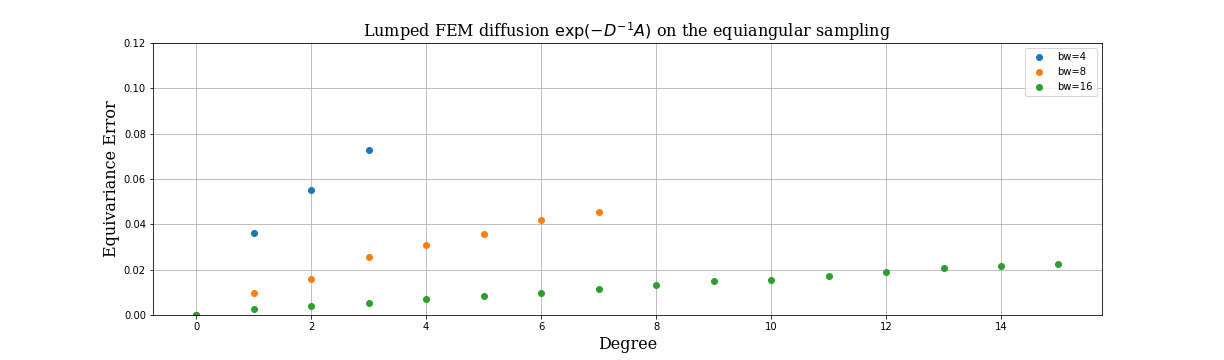
\includegraphics[width=\textwidth]{../codes/06.Equivariance_error/LumpedFEMLaplacianonequiangularsampling.png}
	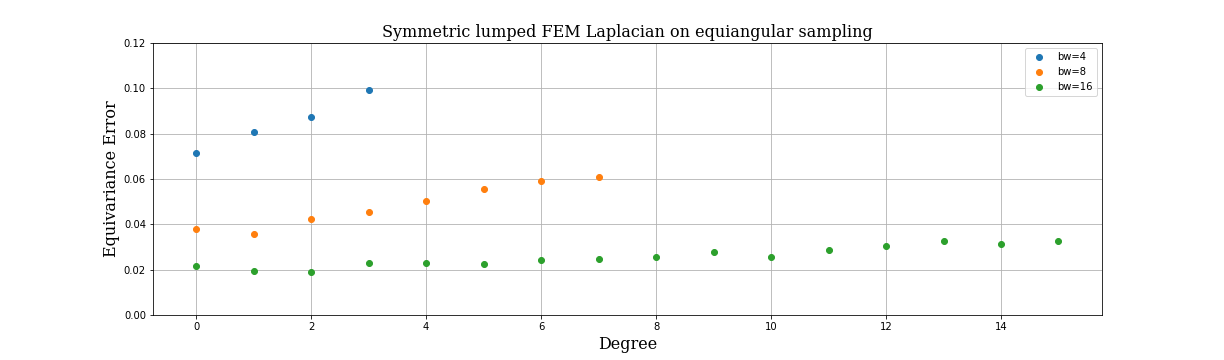
\includegraphics[width=\textwidth]{../codes/06.Equivariance_error/SymmetriclumpedFEMLaplacianonequiangularsampling.png}
	\caption{\label{fig:Equivariance error of the lumped FEM Laplacian}Equivariance error of the lumped FEM Laplacian and of the symmetric lumped FEM Laplacian on the equiangular sampling by spherical harmonic degree $\ell$.}
\end{figure}
\clearpage
\paragraph{Accuracy of the linear FEM spherical harmonics.} Thanks to the sampling theorem \ref{theo:equiangular sampling theorem}, we are able to compute the exact SHT (under the hypothesis of band limited signals) of the solutions to the eigenvalue problem (\ref{eq:algebraic generalized eigenvalue problem}) and we show in figures \ref{fig:FEMHealpix}, \ref{fig:FEMequiangular} the power spectrum of the eigenmodes for both HEALPix sampling and the equiangular sampling, as a measure of the goodness of the linear FEM approach to approximate the spherical harmonics.

\begin{figure}[h!]	
	\centering
	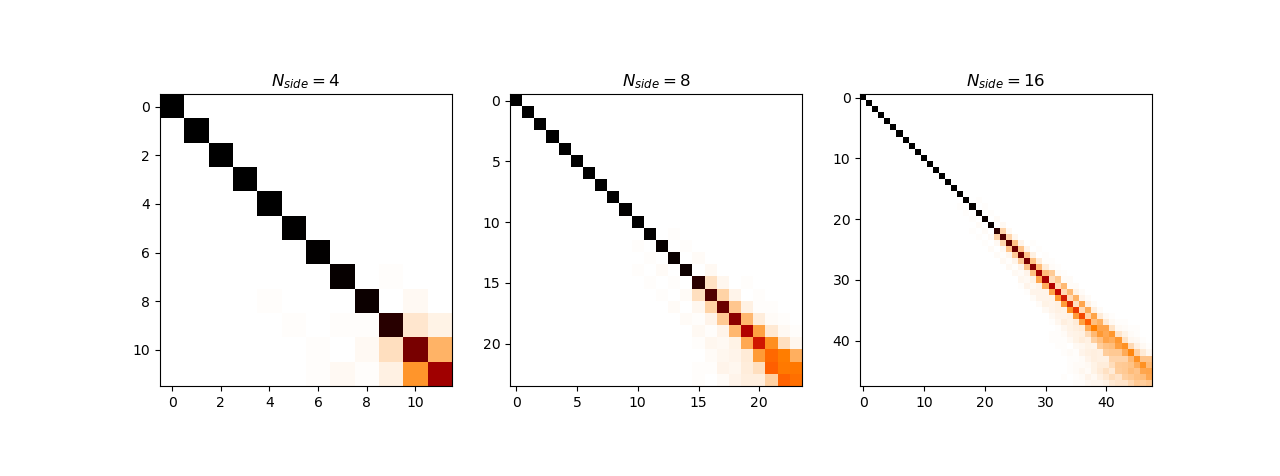
\includegraphics[width=\linewidth]{../codes/03.FEM_laplacian/HEALPix/img/linearFEM.png}\\
	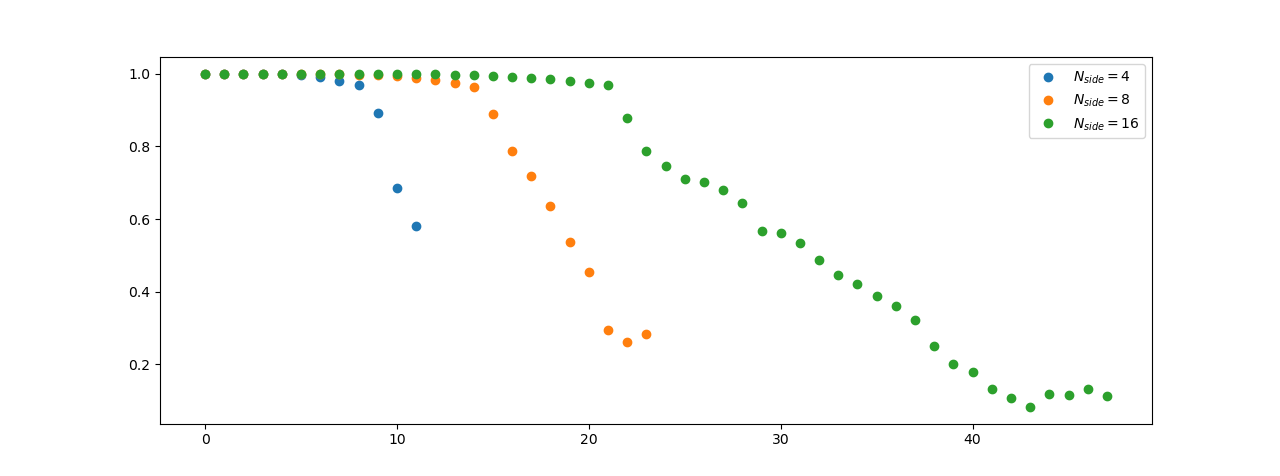
\includegraphics[width=\linewidth]{../codes/03.FEM_laplacian/HEALPix/img/linearFEM_diagonal.png}	\\
	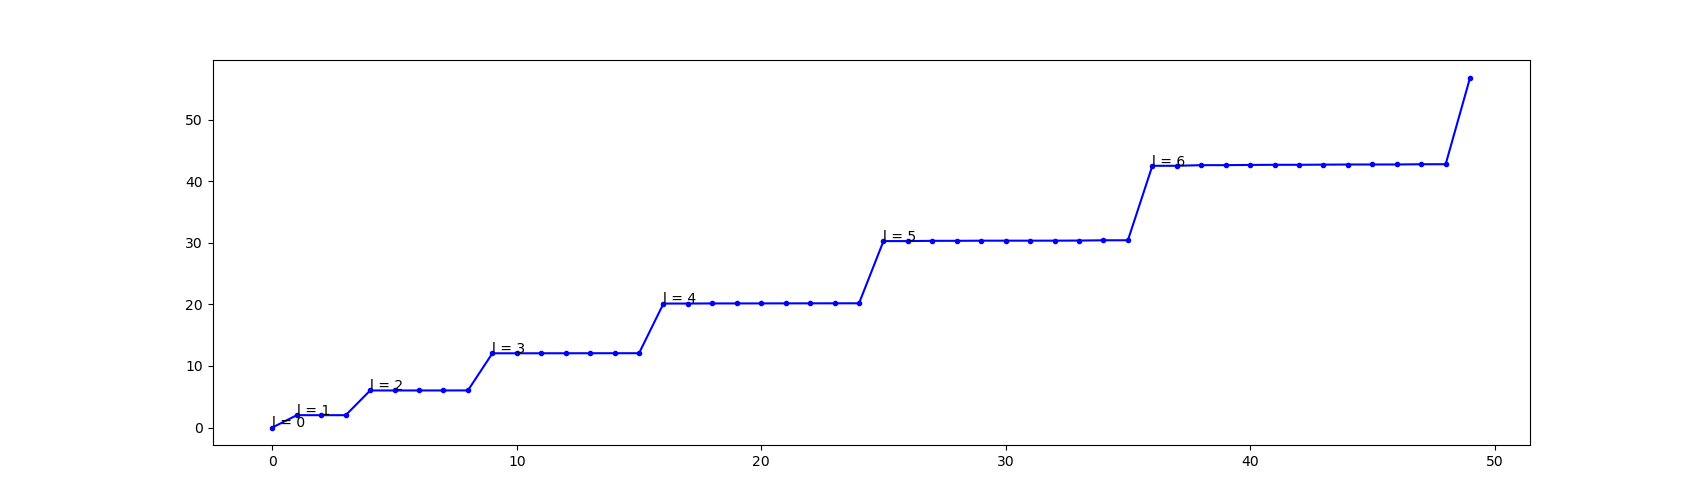
\includegraphics[width=\linewidth]{../codes/03.FEM_laplacian/HEALPix/img/FEM_eigenvalues_16.png}	\\
	\caption{	\label{fig:FEMHealpix}Alignment of eigenspaces of the linear FEM Laplacian on HEALPix, and its spectrum for $N_{side}=16$}
\end{figure}
\begin{figure}[h!]
	\centering
	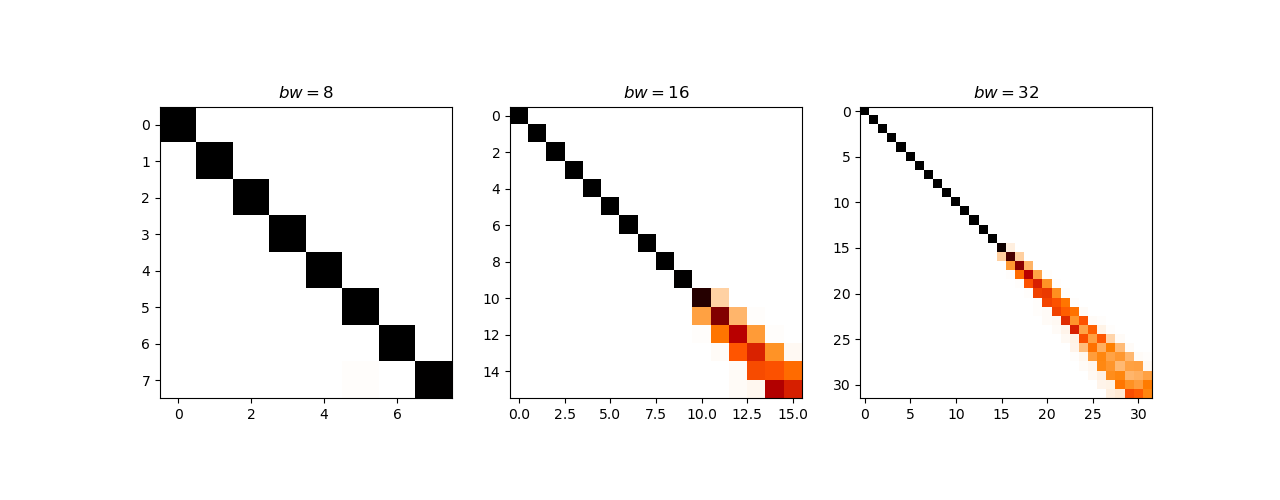
\includegraphics[width=\linewidth]{../codes/03.FEM_laplacian/equiangular/normal/img/linearFEM.png}
	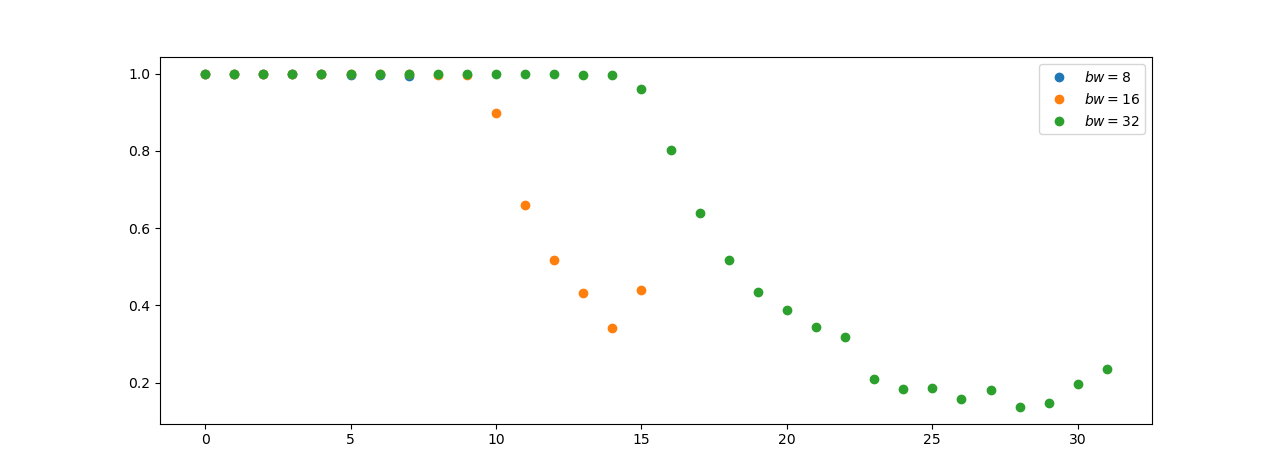
\includegraphics[width=\linewidth]{../codes/03.FEM_laplacian/equiangular/normal/img/linearFEM_diagonal.png}	
	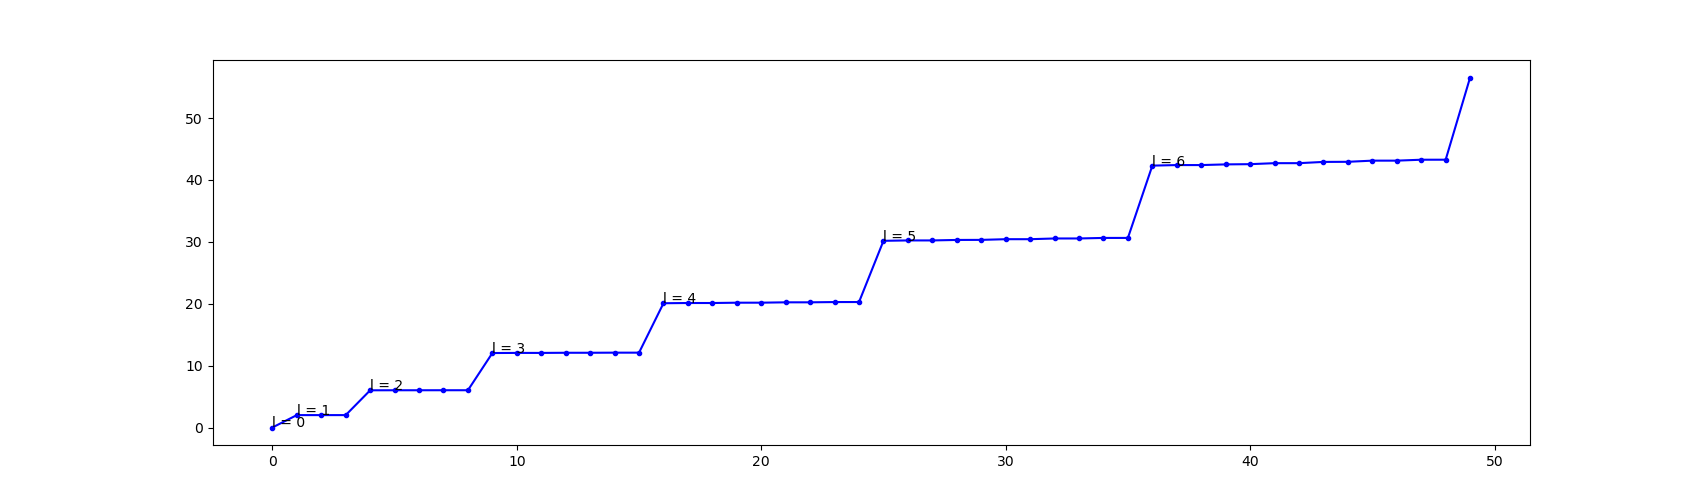
\includegraphics[width=\linewidth]{../codes/03.FEM_laplacian/equiangular/normal/img/FEM_eigenvalues_16.png}	
	\caption{\label{fig:FEMequiangular}Alignment of eigenspaces of the linear FEM Laplacian on the equiangular sampling, and its spectrum for $bw=32$}
\end{figure}

\clearpage






